\section{Views}
In this section, we present three prototypical views that are built upon the
presented visualization infrastructure. The incentive for the users is to
obtain enhanced awareness about available parallelism opportunities. Therefore,
the interaction of the views provide a scalable top-down approach to identify
hotspots, develop parallelization strategies, and validate these strategies for
data dependencies. In the following Sections, we list the suggested views of
this paper.

\subsection{Performance View}
\label{sec:performance_view}
The performance view is a interactive representation of a program's profiling
and trace data. Its primary purpose is to assist users in identifying scenarios
that could potentially improve performance, by employing parallel programming
as an optimization solution. Tracing and profiling provide valuable material
for detailed analysis on how a program behaves at runtime. Presenting a
wholistic view of this data in an easy to digest visualization, can help users
quickly comprehend the program behavior, spot potential performance
bottlenecks, and help guide optimization efforts.

Two visualization modes are provided in the performance view: tracing and
profiling. The tracing mode represents an icicle plot extended with loop
information, i.e., a hierarchical view of calls made during program execution.
The calls are arranged from left to right chronologically, and the visibility
of the loop information for each loop execution can be toggled on or off. The
trace visualization is useful for detailed examination of a program, especially
where the traced invocation order is important. The profiling mode presents the
user a hierarchical view of the functions called during a program's execution.
The length of each function in the view is dictated by the sum of the duration
of calls made to it. The profiling visualization is often sufficient to quickly
pinpoint hot spots.

As user programs grow in size and complexity, the performance data also grows,
and becomes harder to digest all at once. Which is why the performance view
provides zooming on call level and runtime duration filtering, to help the
user adjust the view to different data granularity levels. Runtime duration
filtering sets the minimum runtime duration required for a call to be loaded.
The minimum runtime duration value is gotten by calculating a specified
percentage of the runtime duration of the current top-level call in the view.
This feature allows the render only calls large enough to be easily visible.
With the call zooming feature, users can focus the view on a specific call,
which then makes it the top-level call, re-computes a new minimum runtime
duration, and loads any child calls of the focused call that wasn't visible due
to the previous runtime duration constraint.

\begin{figure*}[ht!]
	\begin{center}
		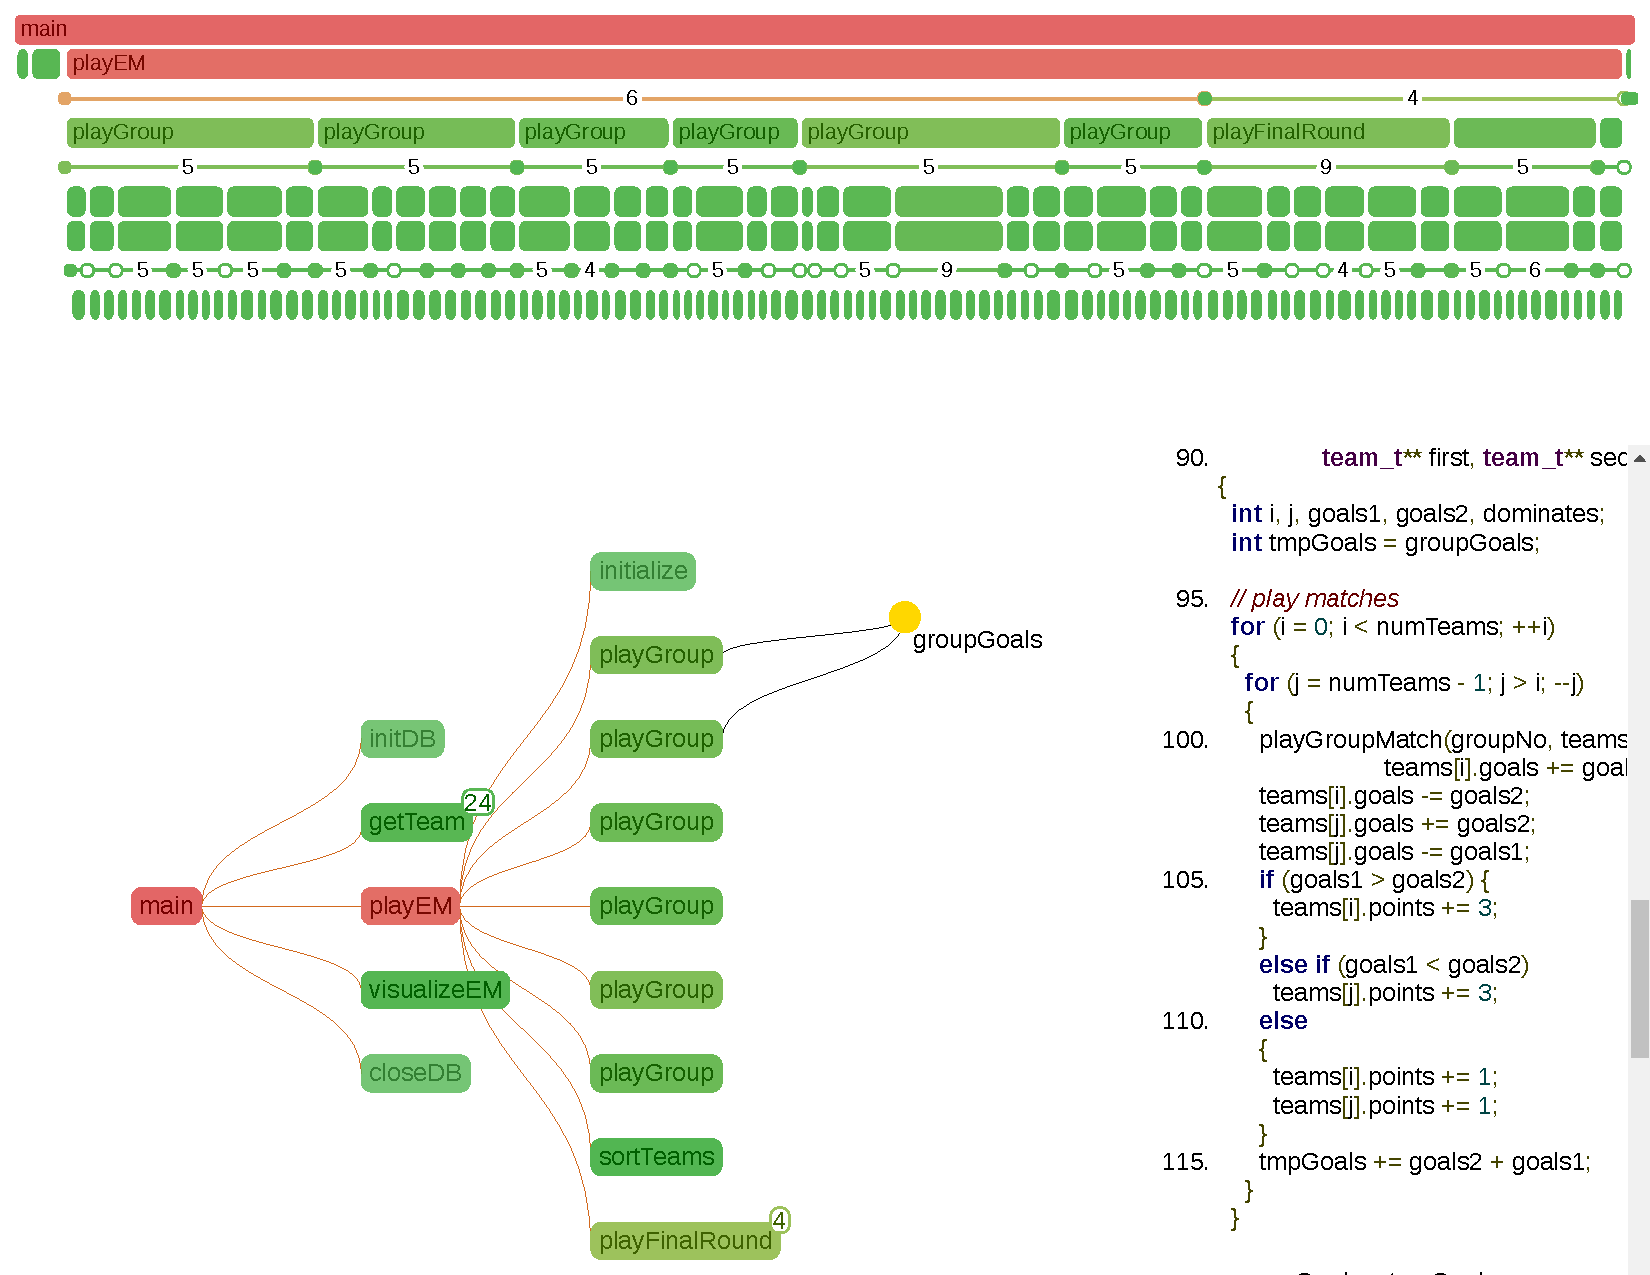
\includegraphics[clip, trim=0.1cm 16.0cm 0.1cm 0.1cm,
width=\linewidth]{img/performance_view.pdf}
		\caption{The performance view of Parceive showing an EMSim trace.}
		\label{fig:emsim}
	\end{center}
\end{figure*}

\subsection{Calling Context Tree (CCT) View}
The CCT view is a visualization that aids the comprehension of dynamic behavior
of an application. The view can display a call tree consisting of call nodes
that is extended with loop nodes and referenced memory nodes (see Figure
\ref{fig:cct_view}). Nodes for calls (or group of calls), loop executions and
loop iterations are positioned using a tidy tree layout~\cite{TidierTree}.
Children of nodes are vertically sorted by their start time to facilitate
comprehension of traced executions. Memory nodes accessed by arbitrary tree
nodes are difficult to integrate as part of a tree layout. Hence, we positioned
these nodes using an unconstrained layout that is based on a force simulation
around the rest of the tree.

The first node present when the view is created is the call to the
\texttt{main} function. Users can arbitrarily expand and collapse call nodes.
When a function was called multiple times during the same function execution,
the respective call nodes are grouped to so-called \textit{call groups}. Call
groups reduce the number of nodes to be displayed but can also be decomposed
into their single call nodes. Navigating loop executions and loop iterations is
similar to calls and allows the user to see information at any desired
granularity. 

For parallelization, the most important feature of the CCT view is data
dependency analysis. Users are often interested in the existence and the
locations of such dependencies between arbitrary regions of their software.
Therefore, a optimized query of the visualization infrastructure is utilized
to detect shared memory accesses across deep call hierarchies. Found
dependencies can then be inspected in a separate source code view. The
described feature allows manageable visualizations by dramatically reducing the
amount of shown nodes. There are some additional features that aim for better
scalability and to help developers parallelizing code:

\begin{itemize}
	\item Profiling information (relative execution time) is present by node
colors.
	\item Exposing and collapsing entity nodes can be performed in both
directions, i.e., to show and hide parent or children nodes.
	\item Seamless zooming or panning, and focusing on single entity nodes for
a clear visualization.
	\item Spotting of arbitrary call nodes that automatically expands the call
tree up to these nodes and start with their common ancestor.
\end{itemize}

\begin{figure}[h!]
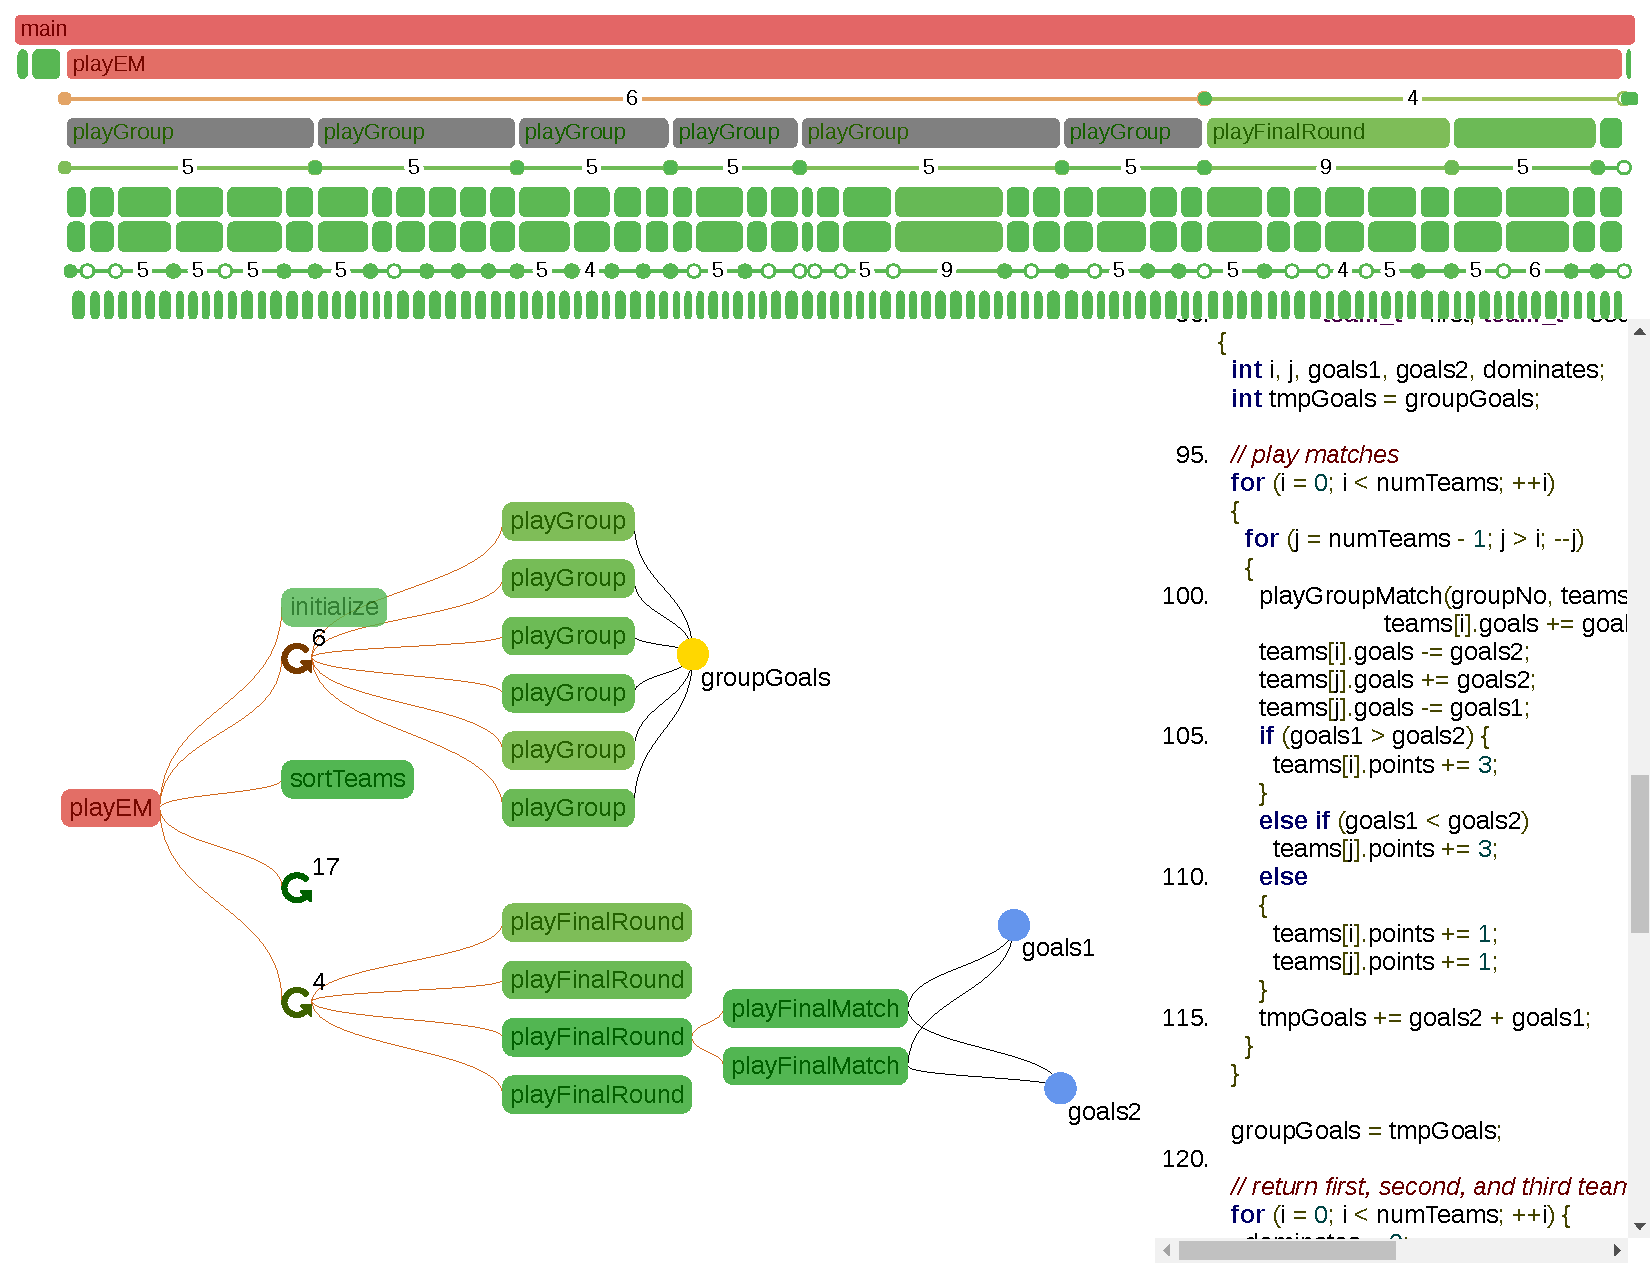
\includegraphics[clip, trim=0.9cm 2.5cm 8.5cm 8.5cm,
width=\linewidth]{img/cct_view}
\caption{The calling context tree view of Parceive.}
\label{fig:cct_view}	
\end{figure}


\subsection{Source View}
The source view shows the highlighted source code in a file that was used to
build the instrumented application.The usefulness of this view becomes apparent
when it is communicating with the others presented in this paper. The simplest
interaction is focusing and it allows the source view to pinpoint the
definition of functions, loops, and memory accesses that makes it easy to
follow the execution of a program trough the source code. Hovering is able to
provide additional information about entities. For calls it can indicate where
the call originated and for memory references where they were allocated and
referenced.